\documentclass[12pt, a4paper, twoside, openright]{report}
% IMPORT SETTINGS
% GENERAL
\newcommand{\thesisType}{M} % M - master, B - bachelor
\newcommand{\thesisAuthor}{David Hambraeus}
\newcommand{\thesisMonth}{\monthname}
\newcommand{\thesisYear}{\the\year}

% Controls e.g. todonotes, front matter, blank pages etc.
\newcommand{\thesisStatus}{f} % d for draft, f for final

% LAYOUT
% One-sided (1) or two-sided (2) layout
% Note: \cleardoublepage is redefed to \clearpage for one-sided layout
\if\thesisStatus f
    \newcommand{\thesisLayout}{2}
\else
    \newcommand{\thesisLayout}{1}
\fi

% TITLE (cover page & title page, imprint page; possibly different line breaks)
\newcommand{\thesisTitle}{Inverse Design of Traveling-Wave\\ Phononic Devices}
\newcommand{\thesisImprintTitle}{Inverse Design of Traveling-Wave Phononic Devices}


% SUBTITLE (cover page & title page, imprint page; possibly different line breaks)
\newcommand{\thesisSubtitle}{}
\newcommand{\thesisImprintSubtitle}{}
% NOTE: Minor modifications are needed if there is no subtitle


% PROGRAMME, DEPARTMENT, DIVISION, RESEARCH GROUP AND UNIVERSITY INFO
\newcommand{\thesisMasterProgramme}{Physics}  % "Master's thesis in \thesisMasterProgramme"

\newcommand{\thesisDepartment}{Department of Microtechnology and Nanoscience}
\newcommand{\thesisDivision}{Quantum Technology Laboratory}
\newcommand{\thesisGroup}{Quantum Photonics Laboratory}

\newcommand{\thesisUniversity}{Chalmers University of Technology}
\newcommand{\thesisUniversityURL}{www.chalmers.se}
\newcommand{\thesisCity}{Gothenburg}
\newcommand{\thesisCountry}{Sweden}
\newcommand{\thesisLocation}{\thesisCity, \thesisCountry}


% MORE IMPRINT PAGE INFO
\newcommand{\thesisSupervisor}{Raphaël van Laer, QPL}
\newcommand{\thesisExaminer}{Raphaël van Laer, QPL}
\newcommand{\thesisPrintedBy}{Chalmers Digital Printing} % remove this line to remove it on the imprint page

\newcommand{\thesisImprintLocation}{SE-412 96 Gothenburg}
\newcommand{\thesisUniversityTel}{+46 31 772 1000}


% COVER FIGURE
% Remove the following line to remove the figure
\newcommand{\thesisCoverFigure}{frontmatter/signed_dist_tmp_254.pdf}
% Caption for cover page figure if used, possibly with reference to further information in the report:
\newcommand{\thesisCoverFigureCaption}{Signed distance field of optimized
level-set beamsplitter design.}

% KEYWORDS
% Comma-separated keywords to appear on abstract page and in pdf info
\newcommand{\thesisKeywords}{%
	phononic devices, quantum acoustics, inverse design, adjoint method,
	level-set, gradient descent, solid mechanics%
}

%encoding
\usepackage[T1]{fontenc}
\usepackage[utf8]{inputenc}
\usepackage{lmodern}

%language
\usepackage[english]{babel}

%paper and text body handling
\usepackage{geometry}
\usepackage{fancyhdr} %Headers and footers
\usepackage{setspace}
\usepackage{lettrine}
\usepackage{glossaries}

%graphics
\usepackage{graphicx}
\graphicspath{{Images/}{./}}
\usepackage[format = plain, labelfont = {bf, it}, textfont = it]{caption}%font settings for captions
\usepackage{xcolor}
\usepackage{pdfpages}
\usepackage{subcaption}
\usepackage{tikz}

%code
%\usepackage{minted}

%math
\usepackage{amsmath}%math
\usepackage{amssymb}%
\usepackage{amsfonts}%
\usepackage{amsthm}%theorems
\usepackage{aligned-overset}
\usepackage{siunitx}
\usepackage{cancel}
\usepackage{braket}
\usepackage{bm}
\usepackage{diffcoeff}
% Use the correct ds in diffs
\difdef{f,s,c}{}{
  op-symbol = \mathrm{d},
}
\difdef{f,s}{f}{
	op-symbol = \delta,
}

%bibliography
\usepackage{csquotes}%for biblatex
\usepackage[
   style = numeric,
   sorting = none,
   date = iso,
   seconds = true
]{biblatex}

%links
\usepackage[colorlinks=true,
            linkcolor=red,
            urlcolor=blue,
            citecolor=gray]{hyperref}

%todo
\usepackage[colorinlistoftodos]{todonotes}


% Temporary (as in for this document only) commands
\newcommand{\fobj}{f_\text{obj}}
%\newcommand{\placeholder}{\boldsymbol{\cdot}}
\DeclareMathOperator{\placeholder}{\boldsymbol{\cdot}}

\newcommand{\todowrt}[2][]{\todo[color=green,inline,#1]{#2}}
\newcommand{\tododec}[2][]{\todo[color=yellow,inline,#1]{#2}}
\newcommand{\todoblk}[2][]{\todo[color=red,inline, #1]{#2}}
\newcommand{\todocit}[2][]{\todo[color=blue!30!white, #1]{#2}}


%special letters
\newcommand{\R}{\mathbb{R}}
\newcommand{\C}{\mathbb{C}}
\newcommand{\Z}{\mathbb{Z}}
\newcommand{\N}{\mathbb{N}}
\newcommand{\F}{\mathcal{F}}
\newcommand{\PP}{\mathbb{P}}
\newcommand{\EE}{\mathbb{E}}

%functions
\renewcommand{\Re}{\textnormal{Re}}
\renewcommand{\Im}{\textnormal{Im}}
\DeclareMathOperator{\Var}{Var} % Variance
\DeclareMathOperator{\Cov}{Cov} % Covariance
\DeclareMathOperator{\Res}{Res} % Residue
\DeclareMathOperator{\Ker}{Ker} % Kernel
\DeclareMathOperator{\tr}{tr} 	% Trace
\newcommand{\scalprod}[2]{\left\langle#1, #2\right\rangle}

% vectors are boldface
\renewcommand{\vec}{\bm}


%settings

%spacing
\renewcommand{\arraystretch}{1.2}
\setlength{\arraycolsep}{3pt}

%units
\sisetup{
   output-decimal-marker = {,},
   exponent-product = \ensuremath{\cdot}
}

\makeglossaries
\newacronym{pml}{PML}{Perfectly Matched Layer}
\newacronym{adam}{ADAM}{Adaptive Moment Estimation}


% CHOOSE SUBSET OF FILES TO COMPILE (USES OLD .aux FILES)
% Sometimes, this will cause a blank page at the beginning.
% One way to fix this is to add \cleardoublepage at the end of every
% included file.
\if\thesisStatus d % only effective in draft mode
    % \includeonly{chapters/methods}
\fi

\begin{document}

% COVER PAGE, TITLE PAGE AND IMPRINT PAGE
\if\thesisStatus f
    \include{template/pages/cover}
\fi
\pagenumbering{roman}
\include{template/pages/title}
\if\thesisStatus f
    \include{template/pages/imprint}
\fi

% ABSTRACT & ACKNOWLEDGEMENTS
\thesisImprintTitle:\\
\thesisImprintSubtitle\\[1ex]
\thesisAuthor\\
\thesisDepartment\\
\thesisUniversity

\thispagestyle{plain}           % Suppress header
\section*{\abstractname}
Phononic devices could enable and improve a broad range of functions in
the realm of quantum computing and sensing as well as classical devices.
However, such devices are currently often designed by hand, combined with brute force
parameter sweeps, which severely limits the designs that can be investigated.
This work presents a method for inverse-design of phononic devices,
allowing a much more general design space to be explored.
At the heart of the method lies a fast calculation of gradients using the
adjoint method, whereby the gradient computation costs no more than a single
normal simulation.
I show that this method is theoretically applicable to phononic devices,
and demonstrate that it works in simulation.
As a proof of concept, I attempt to design a phononic beamsplitter.
The designed devices perform very well, splitting the input power 50/50 with
almost nothing being scattered into other modes or reflected.
However, there are still some complications when transitioning from the first
part of the optimization, with continuously varying material parameters,
to the second part where level-set methods were used to make the design binary.
If these problems can be solved,
this method looks very promising for use in the design of future phononic devices.

\if\thesisType M
    \textbf{Keywords:}
\else
    \textbf{Nyckelord:}
\fi
\thesisKeywords.

% NOTE: this needs modification if the abstract is longer than one page
% (which it shouldn't be)
\if\thesisLayout 2
\newpage                % Create blank page
\thispagestyle{empty}
\mbox{}
\fi

\thispagestyle{plain}           % Suppress header
\section*{Acknowledgements}

First and foremost I would like to thank the members of the Quantum Photonics
Laboratory for making this thesis project possible.
I want to extend a special thank you to Paul and Johan, for their valuable
comments and ideas,
and to my supervisor and examiner Raphaël for fruitful discussions and 


%\vspace{0.25cm}
\hfill
\thesisAuthor, \thesisCity, \thesisMonth\ \thesisYear

% NOTE: this needs modification if there is more than one page of
% acknowledgements (which is probably too much)
\if\thesisLayout 2
\newpage                % Create blank page
\thispagestyle{empty}
\mbox{}
\fi


% CONTENTS LIST (TABLE OF CONTENTS, FIGURES, TABLES)
\include{template/pages/contents}

% BEGINNING OF MAIN DOCUMENT
\pagenumbering{arabic}  % Arabic numbering starting from 1 (one)

\todo[inline]{Todonotes are organized as follows:}
\todo[inline]{General comment / question}
\todowrt{Things that could be done now, no further
simulations/consultation needed}
\tododec{Things that could be done now but I am not sure if I should, or
how to do it}
\todoblk{Things that can't be done yet because they depend on other
things, e.g.\ results}
\todocit[inline]{Citation needed}

\glsresetall
% CHAPTERS
\chapter{Introduction}
\todoblk{After thesis is done, check that I've used cref and not ref}
\todoblk{References before the dot or after? And space or no space?}
\todoblk{ctrl+F for all the times when I write I / we and choose one of them...}
\tododec{Write about why I am using \emph{silicon}}

\tododec{Introduction to quantum acoustics\ldots I need to read more
literature I think}
\tododec{Restructure a little... I would like to talk about inverse design first
and quantum acoustics second. Talk about how inverse design is a concept that
has been applied to nanophotonics but not to quantum acoustics yet. Then talk
about why we care about quantum acoustics. It feels a little bit forced to do it
in that order though, talking about quantum acoustics first might be a better
idea, since that would naturally lead one to introduce the problem of design.}

In recent years, the research into quantum devices of different kinds has
significantly intensified.
Much of it is in one way or another connected to the
construction or operation of a quantum computer.
Though many people are focusing on superconducting circuits, where quanta of
microwave-frequency light are manipulated, there has also been
a growing interest in a different medium for quantum information: sound.
More precisely, acoustic waves in solid materials.
Just like how light, or electromagnetic waves, come in quantized packets of energy called
photons,
so too does acoustic waves and we call those packets phonons.
Just recently, in 2019, researchers coupled an acoustic resonator to a transmon
qubit and were able to directly measure the presence or absence of single
phonons.

Possible applications of quantum acoustic devices, also called phononic devices, are many.
One of them is quantum memory~\cite{sete_high-efficiency_2015}.
Regular computers have both memory and a processing unit that
retrieves data from memory, applies operations on it, and then returns it to
memory.
Keeping all of the data inside the processing unit would be very inefficient,
since the processing unit would then have to be very large.
The same goes for quantum computers: storing all of the quantum information in
the same place where the computation happens is not scalable.
Instead, a quantum memory could be used to store information while it is not
directly needed for the computation.
Another application of quantum acoustics worth mentioning is
coherent transduction between microwave and optical photons.
This would enable communication between physically separated superconducting
circuit based quantum computers~\cite{laer_controlling_2019}.
A third possible application is doing quantum information processing purely in
mechanical elements~\cite{qiao2023developing}.

One important problem with such quantum acoustic devices is that they can be hard to design.
Currently they are often designed by hand,
through analytically motivated guesswork combined with brute force parameter
sweeps.
However, this severely limits the designs that can be investigated.
A parameter sweep of just 6 parameters with 10 different values for each
requires \num{1000000} simulations.
One can of course use smarter optimization algorithms like bayesian optimization
or particle swarm optimization\cite{schneider2019benchmarking,zhang_compact_2013}
to decrease the number of simulations needed, but it will still be of the
same approximate order.

A different approach that has been gaining some popularity in the field of
nano-photonics is \emph{inverse design with adjoint
simulation}~\cite{molesky_inverse_2018}.
The idea is that if the gradient of the figure of merit
with respect to the parameters can be calculated, then we can use gradient based
optimization methods, which converge much faster, even if the number of
parameters is very large. With these methods, one hopes to be able to search
among a much more general class of designs for the optimal one.
This has been successfully applied to photonic devices,
where a wide variety of components have been designed~\cite{spins2019}.
In some cases, for example the waveguide bend, the inverse-designed device could
be made much more compact than conventionally designed
bends~\cite{jensen_systematic_2004}.
In other cases, for example the vertically-incident wavelength-demultiplexing
grating coupler, there are no other known conventional methods of designing the
device~\cite{piggott_inverse_2014}.
However, to our knowledge, no one has yet applied this method to phononic
devices, though there is some work on another type of inverse design of
phononics using machine learning models~\cite{han_deep-learning-based_2022}.


Phononic devices have in general been studied much less than photonic
devices, and the library of known devices is very small.
With this thesis, I explore the possibility of extending the inverse-design paradigm to
quantum acoustic devices.
Since both acoustics and electromagnetics are wave phenomena, there are many
analogies to be drawn, but there are also important differences.
I have in this work shown that the adjoint method is applicable to the case of
acoustics, as well as derived the form of the equations.
As a proof of concept, I attempt to design a phononic 50/50 beamsplitter.
The beamsplitter is conceptually one of the simplest devices imaginable,
and photonic beamsplitters have been studied in great detail for many years
and found a multitude of uses in many different experiments.
However, there is still no standard implementation for phononic beamsplitters,
though \cite{qiao2023developing} has demonstrated a working beamsplitter for
surface acoustic waves.
The two major differences between their design and the one attempted here is
firstly that they are using surface acoustic waves and I am employing bulk
acoustic waves confined in a waveguide, and secondly that their beamsplitter
reflects one of the arms of the beamsplitter back towards the source, whereas I
have one input arm and two separate outputs.

\section{Aim and Thesis outline}

The aims of this thesis are:
\begin{itemize}
	\item Rederive the equations for inverse design with adjoint simulation in
		the case of acoustics and confirm that the methods are theoretically
		applicable.
	\item Implement the methods and use them to design a phononic beamsplitter.
\end{itemize}

Chapter 2 presents some of the theory on solid mechanics and acoustic waves needed to
understand the thesis.
A band diagram over the modes of the waveguide used is also shown there.
In chapter 3, the inverse design process is presented. First, the general
adjoint method is showcased, followed by a derivation in the specific case of
acoustics.
Then, gradient based optimization algorithms are discussed and the ones used in
this thesis are presented.
Chapter 4 describes the specifics of the simulations performed in this work:
both a specification of the skeleton of the devices, how the input wave was excited,
and how the designs were parametrized.


\chapter{Theory}

\section{Acoustic waves and waveguides}

In order to efficiently model the deformation and stresses in a solid material,
a linear elasticity model is often assumed.
For small deformations, solid materials obey Hooke's law which in it's full form
looks like
\[
	\sigma = C : \epsilon
\]
where $\sigma$ is the stress tensor, $C$ the elasticity tensor which is a
four-tensor that is a property of the material,
$\epsilon \coloneqq \nabla \vec u + (\nabla \vec u)^T$
is the strain tensor, and $:$ denotes double scalar product.
This equation is linear in $\vec u$, hence the name \emph{linear} elasticity.
Using this and newtons equations of motion, the equation governing the dynamics
is obtained:
\[
	\rho \ddot{\vec{u}} = \nabla \cdot \sigma + \vec F.
\]
where $\rho$ is the density, $\vec{u}$ is the displacement and $\vec F$ is the
externally applied force.
Assuming a time harmonic solution
$\vec u(\vec x, t) = \vec u(x) e^{i \omega t}$
with angular frequency $\omega$ this becomes
\[
	-\rho \omega^2 \vec{u} = \nabla \cdot \sigma + \vec F.
\]

To combine these into one equation that can be solved for $\vec{u}$ we first
rewrite them in index notation to make calculations clearer:
\begin{align}
	\epsilon_{ij} &= \frac12(\partial_i u_j + \partial_j u_i)\\
	\sigma_{ij} &= C_{ijkl} \epsilon_{kl}\\
				&= \frac12\left(C_{ijkl} \partial_k u_l + C_{ijkl} \partial_l
				u_k\right)\\
				&= C_{ijkl} \partial_k u_l\text{ because of the symmetry of $C$}
\end{align}
which gives
\begin{align}
	F_{i} &= -\rho \omega^2 u_{i} - \partial_j \sigma_{ij}\\
		   &= -\rho \omega^2 \delta_{ik} u_{k} -
		   \partial_j \left(C_{ijkl} \partial_l u_k\right)\\
		   &= -\left(\rho \omega^2 \delta_{ik} \placeholder + 
		   \partial_j \left(C_{ijkl} \partial_l \placeholder\right)\right) u_k
\end{align}
where the indices $i,j,k,l$ go over the spacial dimensions $x,y,z$.
All of the tensors in the equation above are really tensor fields, i.e.\ they are
functions of $\vec{x}$.
Defining the operator $\hat A_{ik}$ as
$-\left(\rho \omega^2 \delta_{ik} \placeholder + 
\partial_j \left(C_{ijkl} \partial_l \placeholder\right)\right)$
we can write
\begin{equation}
	\hat A_{ik} u_k = F_i
\end{equation}

\todowrt{
With no external forces we get traveling modes=eigenvalues.
Explain how and why periodicity means only certain modes can propagate.
Good resource in Chan's thesis, or maybe solid state physics book?
% Bloch state / Bloch's theorem
}

\tododec{At some point write about phonons? I haven't really had to care about
phonons so if I talk about it it's just for applications...}

\todowrt{Show our mode as example of this, and include band diagram}

\todowrt{Write about PML design and why we need it: Simulating infinite
	waveguides isn't possible because of the finite computing power. Also we
don't care about stuff far away, just that there are no reflections that can
interfere. Or maybe write about this in the method\ldots}

\section{Inverse Design}

Inverse design is a design paradigm where the design of a device is guided fully by
the desired characteristics.
These desired characteristics are quantified through what is called an objective
function%
\footnote{
	Also called \emph{figure of merit (FoM)} by some.%
}%
, which I will denote $\fobj$,
that should be maximized.
When coupled with \emph{adjoint simulation}, which is a clever way to compute
gradients, and gradient based optimization
algorithms, this is a very powerful methodology.

An overview of the design process is as follows:
\begin{enumerate}
	\item Initialize a random device design.
	\item\label{it:grad} Calculate the gradient of the design through the adjoint method.
	\item Update the device design using the gradient according to the optimization algorithm.
	\item If the device performance is good enough, terminate optimization, else
		return to step~\ref{it:grad}.
\end{enumerate}

\subsection{Adjoint Simulation}

Adjoint simulation is a way to compute the gradient of $\fobj$ with respect to
the design, which in our case means with respect to the material parameters.
I will in this section first give a general derivation, followed by the case of
inverse design in acoustics.

\subsubsection{General Derivation}\label{sec:general_derivation}

Let $\fobj$ be a function which depends on some (large) vector $v$.
The vector $v$ can be calculated by solving the linear equation
$A v = b$, where $b$ is a fixed vector and $A$ is a matrix that depends on a
vector of design parameters $p$.
The overall goal is to find the parameters $p$ that maximize the objective
function $\fobj$.
The goal of adjoint simulation is to find $\diff{\fobj}{p}$.
This can be expanded through the chain rule as
\[
	\diff{\fobj}{p} = \diff{\fobj}{v} \diff{v}{p}.
\]
To find the latter factor we do
\begin{align*}
	\diff{}{p} [Av = b] &\implies \diff{A}{p} v + A \diff{v}{p} = 0\\
						&\implies \diff{v}{p} = -A^{-1} \diff{A}{p} v
\end{align*}
which gives
\begin{align}
	\diff{\fobj}{p} &= - \diff{\fobj}{v} A^{-1} \diff{A}{p}
	v\label{eq:no_adj_sim}\\
	&= - \left(A^{-T} \diff{\fobj}{v}^T \right)^T \diff{A}{p} v
\end{align}
The first factor of this product is the solution to the \emph{adjoint problem}
\begin{equation}
	A^T \tilde v = \diff{\fobj}{v}^T,
\end{equation}
hence the name adjoint simulation.
As it turns out, $A$ is often symmetric which means that this is simply a normal
simulation but with $\difs{\fobj}{v}^T$ as the source.
Thus, to obtain the derivative we just need to run an additional
simulation with a different input.

Now you might be wondering: what have we gained by this?
Let $n$ be the dimension of $v$, $m$ the dimension of $p$ and $l$ the dimension
of $b$.
This means that $A$ is a matrix with dimension $l\times n$ and $\difs{A}{p}$ is
a three-tensor with dimension $m\times l\times n$.
Thus calculating $A^{-1} \difs{A}{p}$ directly involves solving $Ax = w$ for a
three-tensor, and calculating $A^{-1} \left(\difs{A}{p}\,v\right)$
involves solving for a matrix, both of which are orders of magnitude more
computationally expensive than solving for a vector.

\subsubsection{Specific derivation with acoustics}

Now we turn to the specific case of acoustic devices.
Here $A v = b$ is replaced by the dynamic equation \todowrt[noinline]{dynamic equation?
Better name} of linear elasticity:
\begin{equation}\label{eq:sim_eq}
	\hat A_{ik} u_k = F_i
\end{equation}
Instead of vectors, like we saw in \cref{sec:general_derivation}, these quantities are now functions%
\footnote{%
	Vector-valued funcitons, but that is not the important part here.
}
of $\vec x$.
Analogously to the vector of design parameters we now have a \emph{design field}
$p(\vec x)$.

\begin{tcolorbox}[title=On functionals and their derivatives, breakable,
	parbox=false]
	\tododec{
		Big fat box on functionals and their derivatives. I think this should be
		included somewhere, since very few of my peers know what a functional
		derivative is... Not really sure how though. I kinda like the thought of
		putting it in a box like this 
	}
Our $\fobj$ is no longer a function, but rather a \emph{functional}, and thus
we need to use the functional derivative instead of the ordinary derivative.
One can think of a functional as a function of a function,
i.e.\ something that maps an element of a function space to a scalar number.
There are also functionals which depend on both a function and a real number,
or on multiple functions.
Below I will give an overview of the notational conventions I use,
and then give the definition of the functional derivative as well as some useful
properties of it.

Let $\mathcal{Y}$ be a function space of functions $\R \to \R$.
A functional $F:\mathcal{Y} \to \R$ evaluated at the function
$f\in\mathcal{Y}$
is notated with the function in square brackets: $F[f]$.
If the functional additionally depends on a real number,
$G:\mathcal{Y} \times \R \to \R$,
that is put in round brackets: $G[f](x)$.
Note that in principle, $F$ is the functional while $F[f]$ is just a
number,
analogously to how $f$ is a function while $f(x)$ is a real number.

The functional derivative of $F$ with respect to it's function argument
is a functional $\mathcal{Y} \times \R \to \R$ denoted $\difs.f.{F[f]}{f}$.
In this expression, $f$ is technically a dummy function, writing
$\difs.f.{F[g]}{g}$ is exactly the same functional.
Almost always the functional derivative will be evaluated
at some function $h$.
In the stringent notation this is written
\begin{equation}
	\diff.f.{F[g]}{g} [h]
\end{equation}
and is simply an ordinary function $\R \to \R$.
However, I will use the notation $\difs.f.{F}{h}$ for this, to make the
equations clearer.\footnote{%
	This is consistent with how many other authors use the notation,
	though whether that is an \emph{intentional} notational simplification or
	not I will leave unsaid\ldots
}
\tododec{footnote should probably be deleted\ldots}
In addition, when evaluating the functional derivative at a point, the
argument can be put either after it, or in the denominator:
\begin{equation}
	\diff.f.{F[g]}{g} [h](x) = \diff.f.{F}{h}(x) = \diff.f.{F}{h(x)}.
\end{equation}

The functional derivative is defined by
\begin{equation}
	\int \diff.f.{F}{f} (x) \varphi(x) \dl x
	= \diff*{F[f + \varepsilon \varphi]}{\varepsilon}
\end{equation}
where $F$ is a functional of $f$ and $\varphi$ is an arbitrary test function.
\tododec{I find the definition somewhat difficult to comprehend and really
	didn't understand it until I sat down and did some examples for myself.
	Maybe talk about analogies to vector functions\ldots
}
I will use two properties of the functional derivative:
\begin{itemize}
	\item If $F$ is the functional $F[f](y) = f(y)$,
		then $\difs.f.{F(y)}{f}(x) = \delta(y-x)$.
	\item The chain rule: if $F$ is a functional with one function argument,
		$G$ is a functional with one function and one real argument,
		and $H$ is the functional defined as $H[f] = F[G[f](y)]$,
		then
		\begin{equation}
			\diff.f.{H}{f}(x)
			= \int \diff.f.{F}{G[f]}(y) \diff{G(y)}{f}(x) \dl{y}
		\end{equation}
\end{itemize}
\end{tcolorbox}

\todowrt{Look over what domains all of the integrals integrate over.}

For simplicity I will limit myself to the case where the objective function is
an overlap integral of the displacement field $u_k(\vec x)$ with some function
$\varphi_k^*(\vec x)$:
\begin{equation}
	\fobj[\vec u] = \int u_i(\vec x) \varphi_i^*(\vec x) \dl{\vec x}.
\end{equation}
Such an integral is a scalar product in the space where
$\vec u(\vec x)$ resides.
\tododec[noinline]{This integral would be over the unit cell, or over all of
space but with $\phi_i(\vec{x})$ being non-zero only inside the unit cell}

Analogously to the general derivation, we will use the chain rule to expand
$\difs.f.{\fobj}{p}(\vec x)$.
However, because $\vec u$ is in general complex, I will split it into its real and
imaginary components: $u_i = v_i + i w_i$.
\begin{equation}
	\label{eq:chain_rule}
	\diff.f.{f_\text{obj}}{p}(\bm x)
	=
	\int_\Omega \dl{\bm y} 
	\diff.f.{f_\text{obj}}{v_i}(\bm y)
	\diff.f.{v_i(\bm y)}{p}(\bm x)
	+
	\diff.f.{f_\text{obj}}{w_i}(\bm y)
	\diff.f.{w_i(\bm y)}{p}(\bm x)
\end{equation}
The first factor of each of the two terms is easy enough to calculate:
\begin{align}
	\diff.f.{f_\text{obj}}{v_i}(\bm y) &=
	\diff.f.*{
		\int_\Omega u_j(\bm x) \varphi_j^*(\bm x) \dl{\bm x}
	}{v_i(\bm y)}\\
	&= \int_\Omega
	\diff.f.*{
		u_j(\bm x) \varphi_j^*(\bm x)
	}{v_i(\bm y)} \dl{\bm x}\\
	&= \int_\Omega
	\delta(\bm x - \bm y) \delta_{ij} \varphi_j^*(\bm x)
	\dl{\bm x}\\
	&= \varphi_i^*(\bm y)
\end{align}
and
\begin{align}
	\diff.f.{f_\text{obj}}{w_i}(\bm y) &=
	\diff.f.*{
		\int_\Omega u_j(\bm x) \varphi_j^*(\bm x) \dl{\bm x}
	}{w_i(\bm y)}\\
	&= \int_\Omega
	\diff.f.*{
		u_j(\bm x) \varphi_j^*(\bm x)
	}{w_i(\bm y)} \dl{\bm x}\\
	&= \int_\Omega
	i \delta(\bm x - \bm y) \delta_{ij} \varphi_j^*(\bm x)
	\dl{\bm x}\\
	&= i \varphi_i^*(\bm y)
\end{align}
which gives us
\begin{align}
	\diff.f.{f_\text{obj}}{p}(\bm x)
	&=
	\int_\Omega \dl{\bm y}
	\varphi_i^*(\bm{y})
	\diff.f.{v_i(\bm y)}{p}(\bm x)
	+
	i \varphi_i^*(\bm{y})
	\diff.f.{w_i(\bm y)}{p}(\bm x)\\
	&=
	\int_\Omega \dl{\bm y}
	\varphi_i^*(\bm{y})
	\Re\left(\diff.f.{u_i(\bm y)}{p}(\bm x)\right)
	+
	i \varphi_i^*(\bm{y})
	\Im\left(\diff.f.{u_i(\bm y)}{p}(\bm x)\right)\\
	&=
	\int_\Omega \dl{\bm y}
	\varphi_i^*(\bm{y})
	\diff.f.{u_i(\bm y)}{p}(\bm x)
	\label{eq:dfdp_as_dudp_integral}
\end{align}
\tododec{I am mixing putting the argument in the denominator / after the
functional derivative. Should I be consistent? I like after more, but it is a
bit weird when putting the operant after the derivative}
To find $\difs.f.{u_i(\bm y)}{p}(\bm x)$ we apply $\difs.f.{}{p(\bm x)}$ to
equation~\eqref{eq:sim_eq}, which gives us
\begin{equation}\label{eq:dAdpu_Adudp}
	0 =
	\diff.f.{\hat A_{ik}}{p}(\vec x) u_k(\bm y)
	+
	\hat A_{ik} \diff.f.{u_k(\bm y)}{p(\bm x)}
\end{equation}

The point of inverse design is that we now want to find an ajoint field
$\tilde u_i(\bm y)$
such that the integral in equation~\eqref{eq:dfdp_as_dudp_integral} is
\begin{equation}\label{eq:phi_dudp_integral}
	\int_\Omega \dl{\bm y}\,
	\varphi_i^*(\bm y)
	\diff.f.{u_i(\bm y)}{p}(\bm x)
	=
	\int_\Omega \dl{\bm y}\,
	\tilde u_i(\bm y)
	\hat A_{ik}
	\diff.f.{u_k(\bm y)}{p}(\bm x)
\end{equation}
which by equation~\cref{eq:dAdpu_Adudp} is equal to
\begin{equation}
	\int_\Omega \dl{\bm y}\,
	\tilde u_i(\bm y)
	\diff.f.{\hat A_{ik}}{p}(\vec x)
	u_k(\bm y).
\end{equation}
\todowrt{use the form of $\hat A$ to obtain an explicit formula for this}
The way to find this $\tilde u_i$ is through an adjoint simulation.

\begin{tcolorbox}
	When discretizing space \cref{eq:phi_dudp_integral} becomes
	\begin{equation}
		\varphi_{a}^* \eta_{ab} = \tilde u_{c} A_{ca} \eta_{ab}
	\end{equation}
	Meaning that to find $\tilde u$ we solve
	\begin{equation}
		\varphi_a^* = \tilde u_c A_{ca}
	\end{equation}
	or, taking the hermitian adjoint of both sides
	\begin{equation}
		A_{ac}^\dagger \tilde u_c^* = \varphi_a
	\end{equation}
	which in normal matrix notation is
	\begin{equation}
		A^\dagger \tilde u^* = \varphi
	\end{equation}
\end{tcolorbox}

\todoblk{The infamous integral. Still am not entirely sure about it, but I
haven't thought more about it since I abandoned that.}

\subsection{Optimization Algorithms}

In the last section I painstakingly derived how one can obtain the gradient,
and in this section I will attempt to justify that by describing how one can use
the gradient.
I will begin by describing the advantages of gradient based optimization
algorithms over those that don't use the gradient.
Following that I describe the algorithm that I used, as well as some of it's
predecessors.

An optimization algorithm is an algorithm for finding the optimum of a function.
The function is often called the \emph{objective function} or the \emph{cost
function}.
A very naive optimization method would be to simply try some number of inputs
and then choose the one with the highest function value.
This would require a large number of points before a good value is found,
which means that it would take a long time.
An improvement to this method is to use the information gained from the points
already tried to decide which points to try next.
If some point has a bad value, then try somewhere else; if some point has a good
value, try another close by.
Examples of algorithms that do this are bayesian optimization, particle swarm
optimization, \todowrt[noinline]{more examples}
However, if the input to your function is very high-dimensional,
choosing a random direction step in for your next try is very unlikely
to yield a much better value.
For such functions, it is essential that you know in which direction the
function increases the fastest, so that you can choose your next point in that
direction. That is why we want to use gradient based optimization algorithms;
they enable us to quickly find the right direction to go in for best
improvement.

\tododec{%
	Cool thing to maybe put in. If you have a linear function
	$f(x) = v\cdot x + k$, what is the probability that you will significantly
	(say more than 10\% of optimal step) increase $f$ with a random unit
	length step?
	Optimal: step in $\hat v$, $\Delta f = v\cdot \hat v = \norm{v}$.
	Probability of 10\% of this: $\int_{0.1}^1 (1-x^2)^{n/2} \dl x / \int_{-1}^1
	\cdots$
	use $(1-x^2)^n \approx \exp(-n x^2)$.
}

\subsubsection{Gradient Descent}

The simplest gradient based optimization algorithm is called \emph{gradient
descent}.
Like all of the algorithms I will describe it is an iterative algorithm,
meaning that it generates a sequence of points that converges to an optimum,
and the next point in the sequence is derived from the previous ones.
In the case of gradient descent, the next point is gotten by
\begin{equation}
	p_n = p_{n-1} + \eta g_{n-1}
\end{equation}
where $\eta$ is the so called \emph{learning rate} and $g_{n-1}$ is the gradient
of the objective function at $p_{n-1}$.
For ordinary gradient descent the learning rate would be fixed,
and choosing an appropriate value for this parameter is one of the problems of
this method.
If a too high value is chosen, then the steps taken will be too large and the
optimium might be missed entirely.
A too low value results in too small steps which will yield a slow convergence.

\subsubsection{Adaptive Moment Estimation (ADAM)}

\todowrt{Paragraph describing the \gls{adam} algorithm}

\todowrt{\gls{adam} has one learning rate for each dimension}
\todowrt{\gls{adam} one does not need to manually set the learning rate}
\tododec{Somewhere I should write about epsilon, and alpha and how I set them,
but that probably needs to come later, in the method}

\chapter{Numerical Methods for Acoustic Inverse Design}\label{sec:methods}

% The aim of this thesis is to use inverse design to find a phononic beamsplitter,
% a task that can be divided into three parts: 
% First, some definitions of what
% should be designed and what constitutes a ``good'' design needs to be made.
% Second, a way to calculating the gradient of the ``goodness'' with respect
% to the design is needed.
% And lastly, we need a gradient based optimization algorithm to find the optimal
% design.
% All of this will be described in this chapter.
The aim of this thesis was to use inverse design to find a phononic
beamsplitter. In this section we describe how that was accomplished. First I
specify the skeleton of the device, i.e.\ the parts that were fixed, as well as
the objective function. We then go on to specify how the simulations and
optimization was done.

\section{Design}

The skeleton of the device to be optimized can be seen in \cref{fig:bs-design}.
The input and output waveguides consist of unit cells like the one in
\cref{fig:unitcell}.
The values for the parameters in the sketch are given in \cref{tab:params}.
The reason for using this mode in this waveguide is that it has been shown to be
interesting for avoiding mechanical leakage into the substrate on which it is
clamped, as well as retaining a high optomechanical
coupling~\cite{kolvik_clamped_2023}.

The design placed in the design area was one of two types.
The first was a \emph{continuous design}, meaning that the material parameters
$\rho$ and $C_{ijkl}$ varied continuously. The range of values that they
can take are between the density and elasticity of pure silicon and that of air.
This was parametrized through the \emph{design field}, $p$, which took values
between 0, pure air, and 1, pure silicon.
Any in-between values are not something we can physically realize, but it is
useful as a first step in the optimization. This is because it makes the
optimization landscape smoother which leads to better convergence.
The second kind was a binary design, where each point either had silicon or not
with no in-between values.
This was accomplished using level-set methods, which will be explained in
\cref{sec:level-set}.
Because the device was symmetric, only one half of it needed to be
modeled, and the other half extrapolated through a symmetry boundary condition.

\begin{figure}[htpb]
	\centering
	\def \a{0.5}
\def \w{1.0}
\def \hx{0.13}
\def \hy{0.3}

\tikzset{
	unitcell/.pic={
		\draw[pic actions] (-0.5*\a, -0.5*\w) rectangle (0.5*\a, 0.5*\w);
		\draw[fill=white] (0, 0) circle [x radius=\hx, y radius=\hy];
	}
}

\begin{tikzpicture}[scale=0.7]
	\def \designx{4.0}
	\def \designy{4.0}
	\def \outputh{1.0}
	\def \nunitcells{16}
	\def \nnonpmls{10}

	% Coordinate system
	\draw[gray, thick, ->] (0,0) -- (0,-1) node [anchor=west] {$x$};
	\draw[gray, thick, ->] (0,0) -- (1,0) node [anchor=west] {$y$};

	% Input waveguide
	\path
		(-0.5*\a, 0) pic[transform shape] {unitcell}
		(-1.5*\a, 0) pic[transform shape] {unitcell}
		(-2.5*\a, 0) pic[transform shape] {unitcell}
		(-4.0*\a, 0) node {$\cdots$}
		(-5.5*\a, 0) pic[transform shape] {unitcell}
		(-6.5*\a, 0) pic[transform shape] {unitcell}
		(-7.5*\a, 0) pic[transform shape] {unitcell};
	\draw[red, ultra thick]
		(-7*\a, -0.5*\w) --
		(-7*\a, +0.5*\w);
	\begin{scope}[dash=on 1pt off 1pt phase 0pt]
	\path
		(-8.5*\a, 0) pic[transform shape] {unitcell}
		(-9.5*\a, 0) pic[transform shape] {unitcell}
		(-10.5*\a, 0) pic[transform shape] {unitcell}
		(-12.0*\a, 0) node {$\cdots$}
		(-13.5*\a, 0) pic[transform shape] {unitcell};
	\end{scope}

	% Design area
	\draw (0, -\designx / 2) rectangle (\designy, \designx / 2);
	\node at (\designy / 2, 1) {Design Area};
	\node[left] at (\designy, 0) {$d_x$};
	\node[above] at (\designy/2, -\designx/2) {$d_y$};

	% Output waveguide
	\begin{scope}[xshift=\designy cm, yshift=\outputh cm]
	\path
		(0.5*\a, 0) pic[transform shape] {unitcell}
		(1.5*\a, 0) pic[transform shape] {unitcell}
		(2.5*\a, 0) pic[transform shape] {unitcell}
		(4.0*\a, 0) node {$\cdots$}
		(5.5*\a, 0) pic[transform shape] {unitcell}
		(6.5*\a, 0) pic[transform shape] {unitcell}
		(7.5*\a, 0) pic[transform shape, fill=blue] {unitcell};
	\begin{scope}[dash=on 1pt off 1pt phase 0pt]
	\path
		(8.5*\a, 0) pic[transform shape] {unitcell}
		(9.5*\a, 0) pic[transform shape] {unitcell}
		(10.5*\a, 0) pic[transform shape] {unitcell}
		(12.0*\a, 0) node {$\cdots$}
		(13.5*\a, 0) pic[transform shape] {unitcell};
	\end{scope}
	\end{scope}
	\begin{scope}[xshift=\designy cm, yshift=-\outputh cm]
	\path
		(0.5*\a, 0) pic[transform shape] {unitcell}
		(1.5*\a, 0) pic[transform shape] {unitcell}
		(2.5*\a, 0) pic[transform shape] {unitcell}
		(4.0*\a, 0) node {$\cdots$}
		(5.5*\a, 0) pic[transform shape] {unitcell}
		(6.5*\a, 0) pic[transform shape] {unitcell}
		(7.5*\a, 0) pic[transform shape, fill=blue] {unitcell};
	\begin{scope}[dash=on 1pt off 1pt phase 0pt]
	\path
		(8.5*\a, 0) pic[transform shape] {unitcell}
		(9.5*\a, 0) pic[transform shape] {unitcell}
		(10.5*\a, 0) pic[transform shape] {unitcell}
		(12.0*\a, 0) node {$\cdots$}
		(13.5*\a, 0) pic[transform shape] {unitcell};
	\end{scope}
	\end{scope}
	\draw[|-|]
		(15*\a + \designy, -\outputh) -- node[right] {$s$}
		(15*\a + \designy, \outputh);
		
\end{tikzpicture}

	\caption{
		Device design to be optimized.
		At the red line, a wave traveling right was excited.
		The output was measured over the blue unit cells.
		The dashed unit cells marks \glspl{pml}.
		The large, rectangular design area has dimensions $d_x \times d_y \times
		h$.
	}
	\label{fig:bs-design}
\end{figure}

\begin{table}[htpb]
	\centering
	\caption{%
		Values for the geometric parameters of the device.
		Reference \cref{fig:bs-design,fig:unitcell} for what the quantities
		mean.
	}%
	\label{tab:params}

	\begin{tabular}{cc}
		\toprule
		Parameter & value\\
		\midrule
		$a$ & \qty{187}{\nm}\\
		$w$ & \qty{187}{\nm}\\
		$h_x$ & \qty{153.5}{\nm}\\
		$h_y$ & \qty{49.5}{\nm}\\
		$h$ & \qty{220}{\nm}\\
		$d_x$ & $6 w$\\
		$d_y$ & $4 w$\\
		$s$ & $3 w$\\
		\bottomrule
	\end{tabular}
\end{table}

\subsection{Objective Function}

The figure of merit of the device was the fraction of the input power transmitted
into the output beams.
Furthermore, the power in the output beams was to exit in the same mode as was
excited at the input.
Therefore, a mode overlap integral was used:
\begin{equation}
	I = \int_{\Omega_1} \vec{u}(\vec{x}) \cdot \vec{u}_m^*(\vec{x}) \dl{\vec x},
\end{equation}
where $\vec u_m$ is the shape of the mode (\cref{fig:ms1}).
Because we were not interested in the phase of the output waves,
the absolute value squared of the overlap integral was taken as the objective
function,
\begin{equation}
	\fobj = \abs{I}^2 = I I^*.
\end{equation}
This is maximal when the excitation of the mode $m$ in the output
waveguide is maximized, regardless of which phase it has.
Note that because symmetry is enforced, the power through both outputs will be
the same, and the outgoing waves will have the same phases.

The functional derivative of $\fobj$ with respect to $p$ then becomes
\begin{align}
	\diff.f.{\fobj}{p}(x) &= \diff.f.{I}{p}(x) I^* + I\diff.f.{I^*}{p}(x)\\
	&= \diff.f.{I}{p}(x) I^* + \left(I^*\diff.f.{I}{p}(x)\right)^*\\
	&= 2\Re\left(\diff.f.{I}{p}(x) I^*\right).
\end{align}
The derivative of $I$ was derived in \cref{sec:spec_der}.

\subsection{Excitation}\label{sec:excitation_method}

\tododec{JK thinks a figure or more is apt here?}
\tododec{%
	\emph{%
		RVL: As we discussed once, I feel you actually need more than one
		boundary to excite exactly one mode, or you don't have wavevector
		information on the incoming mode? I presume this is why you get a backward
		propagation mode at excitation point? Please add some explanation.
	}
	\\
	We don't need (and shouldn't have I think) more boundaries. The wavevector
	information is partly given through frequency and partly through the profile
	of the force added. The reason for the backward propagating mode is that the
	boundary stress would be the same for a backward traveling wave. One could
	add a force on the next boundary over to cancel the backward
	propagating wave from the first boundary load, but then that would create
	another backward propagating wave. Perhaps this would be of smaller
	magnitude
}

To excite the input waveguide in the desired mode,
the stress on the boundary of a unit cell was exported from a unit cell
eigenmode simulation with $k=0.9 \pi / a$ and applied to the boundary marked in red in
\cref{fig:bs-design}.
Since the frequency was perfectly controlled, this excites only the desired
mode, since that is the only permitted mode close by as seen in the band diagram
in \cref{fig:banddiagram}.

In order to confirm that the excitation was indeed fully in the desired mode, a
separate model with only a waveguide with 200 unit cells was created.
After applying the excitation and running the simulation,
the proportion of the excitation that ended up in the desired mode was
calculated.
This was done by first calculating the mode overlap integral
$\int \vec u \vec u_m^* \dl{\vec x}$
and comparing that to the norm of the displacement field
$\int \vec u \vec u^* \dl{\vec x}$.
If $\vec u$ is written as $\vec u = a \vec u_m + b \vec u_r$ where $a$ and $b$
are scalars and $\vec u_r$ is orthogonal to $\vec u_m$,
then
$\int \vec u \vec u^* \dl{\vec x} = a\int \vec u \vec u_m^*\dl{\vec x} + b\int
\vec u \vec u_r^*\dl{\vec x}$.
And since $\vec u_r$ is orthogonal to $\vec u_m$,
$a = \int \vec u \vec u_m^*\dl{\vec x} / \int \vec u_m \vec u_m^*\dl{\vec x}$,
which enables us to calculate $b$ as well.
The result was near perfect ($b < 0.03 a$) excitation of only the desired mode.
Since energy is proportional to
the square of the amplitude, $b < 0.03 a$ means that $>99.9 \%$ of the energy was
in the correct mode.
To obtain such high fidelity, it was important that the mesh used for the
unit cells in the wave guide was the same as the mesh in the unit cell
simulation.
High fidelity was also achieved if both meshes were made very fine, but such
fine meshes carries a prohibitively large computational cost.

\subsection{Perfectly Matched Layers (PMLs)}

Ideally, the input and outputs are infinite waveguides.
Unfortunately, infinitely large models require infinite simulation time, which
is problematic.
Instead, \glspl{pml} were placed at the caps of the input and output waveguides.
The purpose of the \gls{pml} was to absorb any incoming waves without reflection,
which would make it act as if there was an infinite waveguide on the other side
into which the waves propagate indefinitely.
One way to accomplish this is to add an imaginary component to the density of
the material.
\todowrt{why does it work}
The imaginary part must be introduced smoothly,
otherwise the abrupt change in material
parameters would induce reflections anyway.
Therefore, the imaginary part was taken to be exponentially increasing,
\begin{equation}\label{eq:rho_im}
	\rho_\text{im} = \rho_\text{si} \cdot s \cdot
	\frac{e^{-\abs{y-y_0} / d} - e^{-n/d}}{1 - e^{-n/d}}.
\end{equation}
In this equation, $y_0$ is the point where the waveguide ends,
$n$ is the length of the \gls{pml}, $d$ decides the steepness of the
exponential and $s$ the final value.
\Cref{fig:pml_profile} shows the effect of changing these parameters on the
shape of the profile of the imaginary component.

\begin{figure}[htpb]
	\centering
	\includegraphics{chapters/methods/pml_profile.pdf}
	\caption{%
		This figure shows the effect of changing the different parameters in
		\cref{eq:rho_im}.
		The green curves shows changing $d$ while keeping the other parameters
		fixed, and the orange and blue show $s$ and $n$ respectively.
		Darker colour means higher value, and the last green curve coincides
		with the first orange, and the last orange with the first blue.
	}%
	\label{fig:pml_profile}
\end{figure}

There are three possible sources of reflections from the \gls{pml} region.
Firstly, if the transition from no imaginary component to some imaginary
component is too abrupt, that causes reflections.
Secondly, if the imaginary component is too small, the waves will not be
completely dampened when they reach the end of the \gls{pml} and thus reflect
off of that.
And lastly, if $d$ is small then there can be reflections from the steep
increase that happens some distance away from the beginning of the \gls{pml}.
See \cref{fig:banddiagram} for an illustration of where the different types of
reflections occur.

\tikzset{
	reflection/.pic={
		\draw[->] (-0.4, 0) -- (-0.1, 0) arc[radius=0.1, start angle=-90, end
		angle=90] --++ (-0.1, 0);
		\draw[dashed] (0,-3.1) -- (0,8.3);
	}
}
\begin{figure}[htpb]
	\centering
	\begin{tikzpicture}[domain=1:8]

		\draw[->,very thick] (-0.0,0) -- (8.2,0) node[right] {$y$};
		\draw[->,very thick] (0,-0.0) -- (0,4.2) node[above] {$\rho_\text{im}$};
		\draw[very thick] (1,0) -- (1,-0.10) node[below] {$y_0-n$};
		\draw[very thick] (7.9,0) -- (7.9,-0.10) node[below] {$y_0$};
		%\draw[very thin,color=gray] (-0.1,-1.1) grid (7.9,3.9);
		\clip (0.0, 0.0) rectangle (7.9,3.9);
		\draw[color=ForestGreen, very thick] (0,0) -- (1,0) --
			plot (\x,{0.40*(exp(\x/3)-exp(1/3))});
		\draw[color=Orange, very thick] (0,0) -- (1,0) --
			plot (\x,{0.10*(exp(\x/4)-exp(1/4))});
		\draw[color=NavyBlue, very thick] (0,0) -- (1,0) --
			plot (\x,{0.02*exp(2.0*(\x-4))});
		\draw[color=Red, very thick] (0,0) -- (1,0) --
			plot (\x,{0.04*(exp(\x/2)-exp(1/2))});
		\draw[ForestGreen] (1.0, 0.3) pic {reflection};
		\draw[NavyBlue] (5.7, 0.8) pic {reflection};
		\draw[Orange] (7.9, 0.9) pic {reflection};
	\end{tikzpicture}
	\caption{%
		For the green curve, the initial sudden increase of the imaginary
		component of the density at the beginning of the \gls{pml} causes reflections.
		For the blue curve, the beginning of the \gls{pml} is smooth but there
		is an increase partway through sharp enough to cause reflections.
		For the orange curve, the \gls{pml} never becomes strong enough to
		completely dampen the waves, and they get reflected at the end.
		The red curve balances all these, yielding a perfect, reflectionless
		\gls{pml}.
	}%
	\label{fig:pml_reflections}
\end{figure}

It was desirable to make $n$ as small as possible while still eliminating all
reflections.
This was because a smaller $n$ meant a smaller model which resulted in shorter
simulation times.
In order to do so, a long waveguide with the same parameters as
used for the input and output waveguides in the beamsplitter design was created.
To discern where there was some component of the wave reflected, a fourier
transform of the displacement field was made.
The parameters controlling the shape of the $\rho_\text{im}$ curve were then
varied and an appropriate value was selected.

\subsection{Level-Set}\label{sec:level-set}

Ultimately, we wanted the device to consist of regions of material and regions of
no material.
Such a design is defined by the boundary between filled and empty regions.
How to best implement a method of storing and evolving this boundary requires
some thought.
The first, and perhaps most intuitive implementation,
would be to simply store the coordinates of evenly spaced points on the boundary.
In addition to storing the coordinates, one must also store which points
neighbour which.
A different method, which is the one used in this report, is called
the \emph{level-set method}.
With this method, the boundary is not directly stored, but is rather stored via an
\emph{implicit function}, $\phi(x)$,
and the boundary is recovered as the
0-isocontour of $\phi$, i.e.\ the points $x$ where $\phi(x)=0$.

There are two main advantages of using the level-set method rather than
directly storing the boundary points.
Firstly, when moving the boundary we would like to do so in the normal
direction, as moving it along itself has no effect.
Computing the normal direction of a directly stored boundary is slightly cumbersome,
though certainly achievable.
With level-set, moving the boundary in the normal direction is as easy as adding
a constant to the implicit function.
Secondly, while the boundary is changing, the resolution in one part might need
to be increased while the resolution in another needs to be decreased. Deciding
where and when to add new points is non-trivial when directly storing the
boundary. Furthermore, if two domains merge, or if one splits, points
need to be removed and the connectivities changed, which is difficult.
\Cref{fig:direct_troubles} illustrates these problems with direct storage concretely.
Both of these issues are automatically handled with the level-set method, as
shown in \cref{fig:signed_dist_example}.

\begin{figure}[htpb]
	\centering
	\begin{tikzpicture}[scale=1.5, very thick]
	\coordinate (ca) at (0,0);
	\coordinate (cb) at (1,0);
	\def\radiusa{0.7cm}
	\def\radiusb{0.1cm}
	\def\radpt{0.7pt}
	\draw (-1,-1) rectangle (1.5,1);
	\foreach \i in {0,15,...,360}{% 
		\filldraw [blue]  (ca)++(\i:\radiusa) circle (\radpt);
	}
	\foreach \i in {0,72,...,360}{% 
		\filldraw [blue]  (cb)++(\i:\radiusb) circle (\radpt);
	}
	\draw (ca) circle[radius=\radiusa];
	\draw (cb) circle[radius=\radiusb];

	\begin{scope}[xshift=3cm]
		\coordinate (ca) at (0,0);
		\coordinate (cb) at (1,0);
		\def\radiusa{0.4cm}
		\def\radiusb{0.4cm}
		\draw (-0.8,-1) rectangle (1.7,1);
		\foreach \i in {0,15,...,360}{% 
			\filldraw [blue]  (ca)++(\i:\radiusa) circle (\radpt);
		}
		\foreach \i in {0,72,...,360}{% 
			\filldraw [blue]  (cb)++(\i:\radiusb) circle (\radpt);
		}
		\draw (ca) circle[radius=\radiusa];
		\draw (cb) circle[radius=\radiusb];
	\end{scope}
	\begin{scope}[xshift=6cm]
		\coordinate (ca) at (0.2,0);
		\coordinate (cb) at (0.8,0);
		\def\radiusa{0.4cm}
		\def\radiusb{0.4cm}
		\draw (-0.8,-1) rectangle (1.7,1);
		\foreach \i in {60,75,...,315}{% 
			\filldraw [blue]  (ca)++(\i:\radiusa) circle (\radpt);
		}
		\foreach \i in {-72,0,72}{% 
			\filldraw [blue]  (cb)++(\i:\radiusb) circle (\radpt);
		}
		\foreach \i in {-45, -30, ..., 45}{% 
			\filldraw [red]  (ca)++(\i:\radiusa) circle (\radpt);
		}
		\foreach \i in {144, -144}{% 
			\filldraw [red]  (cb)++(\i:\radiusb) circle (\radpt);
		}
		\draw (ca)++(60:\radiusa)
			arc[radius=\radiusa, start angle=60, end angle=300]
			to[out=30, in=150]
			([shift=(240:\radiusb)] cb)
			arc[radius=\radiusb, start angle=240, end angle=480]
			to[out=210, in=-30]
			cycle;
		%\draw (cb) circle[radius=\radiusb];
	\end{scope}
\end{tikzpicture}

	\caption{%
		Possible evolution of boundary. In the leftmost figure, the
		boundary is defined by pretty much evenly spaced points. In the center figure
		the boundaries have moved and the spacing is no longer even, and the
		right circle is very poorly resolved.
		The rightmost figure shows the boundary after the two circles moved
		closer together. Now there are multiple points that need to be removed,
		marked in red, and the connectivity of the points that remain must be
		changed such that the two boundaries are merged.
	}%
	\label{fig:direct_troubles}
\end{figure}
\begin{figure}[htpb]
	\centering
	\includegraphics{chapters/methods/signed_dist_example.pdf}
	\caption{%
		Signed distance function for the boundaries in
		\cref{fig:direct_troubles}. The resolution of the boundary depends only
		on the resolution of the signed distance field, and not on how the
		boundary moves, so evolving boundaries will never become poorly
		resolved. Additionally,
		topological changes are also smoothly handled since there is no need to
		explicitly specify connectivities.
	}%
	\label{fig:signed_dist_example}
\end{figure}

There are of course a lot of possible functions $\phi(x)$ that have a given
boundary as it's 0-isocontour.
There is one choice that simplifies a lot of calculations though: the signed
distance function.
This function is defined as the distance from the closest point on the boundary,
with a plus sign if it is inside and a minus sign if it is outside the boundary.
See \cref{fig:signed_dist_example} for an example.
It has the advantage that if one wishes to locally shift the boundary some
length $s$ in the normal direction, then simply add $s$ to the function there.
\Cref{fig:add_shift} shows this effect in one dimension.
\todowrt{%
	Create another figure that shows it in two dimensions.
	I'm thinking a circular boundary, and adding $s$ in the left half and
	subtracting $s$ in the right half. Alternatively adding $s\cdot x$ (unit circle
	centered on 0) so that it will be smooth
}

\begin{figure}[htpb]
	\centering
	\begin{tikzpicture}[domain=0:3]
		\draw[very thin,color=gray] (-0.1,-2.1) grid (2.9,1.9);

		\draw[->] (-0.2,0) -- (3.2,0) node[right] {$x$};
		\draw[->] (0,-2.2) -- (0,2.2) node[above] {$\phi$};
		\draw[color=blue!50, dashed, very thick] plot (\x,{\x-2})
			node[right] {$\phi(x)$};
		\draw[color=blue, very thick] plot (\x,{\x-1})
			node[right] {$\phi(x)+s$};
		\filldraw[color=blue!50] (2,0) circle[radius=2pt];
		\filldraw[color=blue]    (1,0) circle[radius=2pt];
		\draw[color=red, ->, very thick] (1.9,0) --
			node[below] {$s$}
			(1.1,0);
	\end{tikzpicture}
	\caption{Adding $s$ to the signed distance function shifts boundary by
	$s$.}%
	\label{fig:add_shift}
\end{figure}

Using a signed distance function means that a gradient descent step could be taken
by simply adding the gradient field to the signed distance field.
However, there are some pitfalls that had to be avoided.
Firstly, the gradient needed to be rescaled so that the boundary moved
an appropriate distance.
This was done such that the boundary moves at most \qty{1}{\nm}.
\todoblk[noinline]{check this number before finalizing, we change it every now and then}
Secondly, since the gradient was occasionally sharply peaked somewhere
far from the boundary, only the gradient near the boundary is actually added
to the signed distance field.
After performing this addition, what was previously a signed distance field
would now no longer be that, and thus the signed distance field was recalculated from
the new, shifted boundary.
This recalculation came with a performance penalty, but since the COMSOL
simulations were orders of magnitude slower than all other parts of the
optimization, this was of little concern.


\section{Optimization}\label{sec:m_optimization}

For the optimization, we used the \gls{adam}
algorithm with one modification:
a global learning rate was employed rather than
separate learning rates for each dimension.
The reasoning for this was that separate learning
rates would give jagged contours, which might not be properly resolved by the
meshing. Practically this modification means that \mintinline{Python}+v+ is a
scalar and is set to \mintinline{Python}{(1-beta_2)*np.mean(g**2) + beta_2 * v}
in \cref{lst:adam}.
The optimization was run and continually monitored, and once convergence was
visually confirmed through looking at the plot of $\fobj$ by iteration, it was terminated.
A few different values for the $\beta$:s were tried, and in the end
$\beta_1=0.9$ and $\beta_2 = 0.95$ were chosen.
However, it seemed that the evolution were not too sensitive to this choice.
$\alpha$ was taken to be \num{2e-3}, because that is large enough that $p$
could change from 0 to 1 in 500 iterations, which was deemed an appropriate
timescale as the time per iteration was about 4 minutes.
A too large $\alpha$ would lead to poor convergence, while a too low value would
result in slow progress.

The final step of the optimization was to use level-set for the design.
However, just using the $p=0.5$ boundary of the final optimized continuous
design as the initial point of the level-set optimization would be an abrupt
change, and there is no reason to expect that the resulting level-set design
would be close to a design with good performance.
Therefore, once the continuous optimization had converged, a sigmoid function
was applied to the design field $p$ before $\rho$ and $C_{ijkl}$ were set:
\begin{align}
	\rho(\vec x) &= \rho_\text{si} \sigma_r(p(\vec x)),
	&
	C_{ijkl}(\vec x) &= C_{ijkl}^\text{si} \sigma_r(p(\vec x)),
	&
	\sigma_r(p) = \frac{1}{1+e^{-(p-0.5)/r}}.
\end{align}
and then the optimization was restarted.
The sigmoid results in fewer values close to 0.5, effectively making the device
closer to being binary, which means that the step to level-set designs wasn't as
abrupt.
Note that the parameter $r$ controls how much values are shifted, and with
$r\to 0$, $\sigma_r$ becomes a step function.
Once that had been repeated a couple of times with decreasing $r$,
the level-set design was
initialized using the $p=0.5$ boundary of the final optimized design,
and the level-set optimization was run.

\section{Simulations}

In this section we detail some of the practicalities of performing the
simulations.
For finite element simulations we used COMSOL version 6.0.
First, a unit cell with periodic boundary conditions was simulated,
from which we obtained:
\begin{itemize}
	\item the mode shape, used to calculate the component of the displacement
		field in the desired mode,
	\item the stress at the boundary, used as the force exciting the input
		waveguide,
	\item the frequency at which to excite in order to obtain a traveling wave
		with the desired wave vector.
	\item a mesh to be used when meshing the unit cells in the waveguides.
\end{itemize}

For the continuous optimization, the basic procedure went
\begin{enumerate}
	\item Through the COMSOL-Matlab API, a beamsplitter model was made.
		The excitation force profile as well as the unit cell mesh and the mode
		shape were imported from the unit cell simulation.
	\item A semi-random initial design field $p$ was created. This was done by
		drawing a sample from a Gaussian process, which means that the characteristic
		length scale that the design varies on could be controlled.
	\item\label{it:sigmoid} If the sigmoid function was to be used in this optimization, it was
		applied to the design field, and the result was saved to a different
		variable, that we call the interpolation field.
	\item The interpolation field was imported to the COMSOL model, and the
		material parameters adjusted proportional to said field.
	\item Both forward and backward simulations were run and the gradient was
		calculated and exported to Matlab.
	\item With the gradient, the design field was updated and the algorithm
		returned to step~\ref{it:sigmoid}.
\end{enumerate}

For the level-set optimization, the procedure was basically the same, with some
minor differences:
\begin{enumerate}
	\item Through the COMSOL-Matlab API, a beamsplitter model was made.
		The excitation force profile as well as the unit cell mesh and the mode
		shape was imported from the unit cell simulation.
	\item An initial signed distance field $s$ was created.
		This was done by finding the $p=0.5$ isocontour from the final iteration
		of the continuous optimization, and initializing a signed distance field
		from that.
	\item\label{it:import} The zero isocontour of the signed distance field was imported into
		the COMSOL model and a geometry was built from that.
	\item Both forward and backward simulations were run and the gradient was
		calculated and exported to Matlab.
	\item With the gradient, the signed distance field was updated and the algorithm
		returns to step~\ref{it:import}.
		Note that as part of the update, the signed distance field was
		reinitialized so that it would not lose its properties.
\end{enumerate}

\chapter{Results and Discussion}

In this chapter I present and discuss the results of my work.
The first section, \cref{sec:long_waveguide}, presents the simulations needed to
ascertain that the beamsplitter simulations would work as intended.
This includes tuning the \gls{pml} parameters and checking that the excitation
excites the right mode.
After that, I present the results of the continuous optimization followed by the
results for the level-set optimization in \cref{sec:res_cont,sec:res_bin}
respectively.
In summary, the continuous optimization yielded near perfect devices with full
transmission and very little reflection.
The level-set optimizations never reached quite as good performance, with around
10\% of the power getting reflected.
\todoblk{BUT IT IS STILL INCREASING!}
% The continuous optimization efforts was plagued by a persistent failure to
% converge, and thus a large part of my work was to try to solve this.
% This failure to converge prevented a gradual shift toward binary devices,
% which would have allowed for a smoother transition to the
% level-set design paradigm.
% Nevertheless, the level-set methods were also tried,
% but with either manually set starting points or suboptimal designs seen in the
% continuous optimization.
% Finally, the continuous optimization did converge and yielded devices which
% transmitted approximately 95 \% of the incoming waves.

\section{Long waveguide simulations}\label{sec:long_waveguide}

As detailed in \cref{sec:methods}, a long waveguide without any beamsplitter
elements was simulated to ascertain that the excitation method correctly excited
only the desired mode, and that the \gls{pml} elements were reflectionless.
In this section I present the results from those simulations.
The waveguide used for these is pictured in \cref{fig:long_waveguide}

\begin{figure}[htpb]
	\centering
	\includegraphics[width=\textwidth]{chapters/results/long_waveguide_geom.png}
	% \includegraphics[width=\textwidth]{chapters/results/long_waveguide_v_d=5_s=0.02.png}
	% \includegraphics[width=\textwidth]{chapters/results/long_waveguide_selections.png}
	\caption{%
		This figure shows the long waveguide used for the \gls{pml} simulations
		as wells as validating the excitation method.
	}%
	\label{fig:long_waveguide}
\end{figure}

\subsection{Excitation}

The fact that the excitation was almost solely in the desired mode was verified
in two ways.
Firstly, as detailed in \cref{sec:excitation_method}, $a$ and $b$ in $u = a u_m
+ b u_r$ was computed.
The result was that $a = 1.166$ and $b = 0.0327$.
Thus $99.92\%$ of the energy was in the desired mode.
Secondly, a fourier transform of the y-component of the displacement field was
made.
This can be seen in \cref{fig:v_ft}.
The other modes that could be excited at this frequency have very different wave
vectors, which means that they would show up as separate peaks somewhere around
$0.4 \pi / a$ and $0.1 \pi / a$.
Since no other peaks can be seen, this further supports the result that only the
desired mode is excited.

\begin{figure}[htpb]
	\centering
	\includegraphics{chapters/results/ft_figure.pdf}
	\caption{%
		Fourier transform of the y-component of the displacement field.
		It clearly shows one wave traveling forward with a k-vector of
		$0.9 \pi / a$, where the dashed gray line is.
		Since the closest other mode at this frequency is at
		$k_y \approx 0.4 \pi / a$, where no peak is visible, it is concluded
		that solely the desired mode is excited.
	}%
	\label{fig:v_ft}
\end{figure}

\subsection{PML investigation}

\Cref{fig:pml_sweep1} shows the amplitude of the reflection,
quantified as the peak height relative to the forward propagating wave,
for different profiles.
These figures fit well with the three types of reflection mentioned previously.
The leftmost plot in \cref{fig:pml_sweep_sd} shows that all of the different
shapes yield reflections when the derivative at the beginning of the \gls{pml}
is around \num{3e-4}, which indicates that the reflections are dominated by
effects from the sudden start of the \gls{pml}.
On the other end, the increase in reflection amplitude come from
waves reaching the end of the \gls{pml} and getting reflected there.
The third type of reflection seems to only be noticeable for $d \leq 4$.
It is also worth noticing that with lower $d$, the plateau where neither of the
first two kinds of reflections are significant is broader.
Since $d=5$ was the lowest $d$ to show no signs of the third type of reflection,
that was chosen for the shape of the \gls{pml} profile.
After that, we investigated how short we could make the it while retaining
low reflections. \Cref{fig:pml_sweep_sn} shows $s$ sweeps for different $n$.
To achieve a short yet functional \gls{pml}, $d=5$, $s=0.03$ and $n=20$ was
chosen.
For $n=15$, reflections from the beginning start to become significant before
the reflections from the end have waned.

\begin{figure}[htpb]
	\centering
	\begin{subfigure}[]{0.99\textwidth}
	\begin{center}
		\includegraphics{chapters/results/pml_sweep_sd.pdf}
	\end{center}
	\caption{
		On the left is the reflection amplitude plotted as a function of the
		\gls{pml} strength $s$ for different $d$.
		For $d > 4$ there are two sources of reflection:
		for small $s$ reflection at the end of the \gls{pml} occurs,
		and for large $s$, there is reflection at the beginning.
		The right figure makes it clear that it is the slope at the beginning of
		the \gls{pml} that matters, since the point at which it becomes
		significant is the same for all $d$.
	}
	\label{fig:pml_sweep_sd}
	\end{subfigure}%

	\begin{subfigure}[]{0.99\textwidth}
	\begin{center}
		\includegraphics{chapters/results/pml_sweep_sn.pdf}
	\end{center}
	\caption{
		This is the same as \cref{fig:pml_sweep_sd} but with varying $n$.
		For $n=15$, the reflections from the beginning do not subside before the
		reflections from the end become significant, so at least $n=20$ is
		necessary.
	}
	\label{fig:pml_sweep_sn}
	\end{subfigure}
	\caption{}
	\label{fig:pml_sweep1}
\end{figure}

\section{Continuous optimization}\label{sec:res_cont}

There was a lot of problems with the optimization of the continuous design.
Many optimization runs would end up looking like \cref{fig:bad_cont_conv},
reaching a somewhat performant beamsplitter but invariably declining after some
point.
The figure shows the evolution of the transmitted power in one of the
output arms, as well as the reflected power back into the input.
This has been normalized such that 1 is the power in through the input waveguide.
Thus, an optimal beamsplitter would reach 0.5.
If the powers do not add up, it is because energy is flowing out in a different
mode.
I tested a few different theories on why the algorithm might fail to converge.
The first one was that perhaps the simulations were unstable for the case when
$p\approx 0$. To test this I interpolated between $\rho^\text{si}$ and
\qty{1000}{\kg\per\m^3} instead. However, convergence was still not reached.
The second was that maybe the meshing was too coarse to resolve the design
field properly. However, this was not the case as increasing the meshing did not
change the objective function more than a percent or so, so this wasn't the
cause either.
The last thing I thought of was that comsol was using quadratic shape functions
for the fields. This means that on each finite element of the mesh, the fields
are approximated with quadratic polynomials. Thus, if one computes any third
order spatial derivative, it will be 0 everywhere, and the second order
derivatives will not be very accurate.
In \cref{fig:quad_spline_sine} I show how quadratic splines can give a very good
approximation to a function, while still being a terrible approximation to its
second derivative.
Since I used second derivates in computing my gradient, that also wasn't very
reliable.
One way of solving this is to use higher order shape functions, however this
greatly increases the degrees of freedom, making the problem too computationally
expensive, at least with our hardware and geometry.
Another way is to make the mesh much finer, but this is also too computationally
expensive.
\begin{figure}[htpb]
	\centering
	\includegraphics{chapters/results/quad_spline_sine.pdf}
	\caption{%
		This figure shows a quadratic spline approximation to a sine function,
		given eight points on the function. Even though the spline approximates
		the sine function very well, the second derivative approximation is
		terrible.
	}%
	\label{fig:quad_spline_sine}
\end{figure}

However, there was another way:
using the built in COMSOL function \mintinline{c}+fsens+ for computing
the gradient, convergence was obtained.
\Cref{fig:cont_conv1} shows the performance evolution of this optimization run.
At iteration 467, the model was deemed to have converged and as described in
\cref{sec:m_optimization}, a sigmoid function with $r=0.1$ was applied and optimization
continued.
At iteration 615, the model again seemed converged and $r$ was set to $0.05$.
Finally, at iteration 830, near perfect performance was reached and optimization
was terminated.
\Cref{fig:cont_design1} shows the design field after convergence for each of the
three stages.

\begin{figure}[htpb]
	\centering
	\includegraphics{chapters/results/conv_22.pdf}
	\caption{%
		Non-converging optimization example. The blue curve shows the
		transmitted power in one of the output arms as a function of iteration,
		while the yellow shows the power reflected back out through the input.
		The cases where two times the blue plus the yellow isn't 1.0 is
		explained by power exiting through a different mode.
	}%
	\label{fig:bad_cont_conv}
\end{figure}

\begin{figure}[htpb]
	\centering
	\includegraphics{chapters/results/conv_31.pdf}
	\caption{
		Similar to \cref{fig:bad_cont_conv},
		but at iteration 467 and 615, a sigmoid function was abruptly applied
		to the design field, which causes the dips.
		The final device was a near perfect beamsplitter, with less than 1 \% of
		the power begin reflected, and nothing being scattered into other modes.
	}%
	\label{fig:cont_conv1}
\end{figure}

\begin{figure}[htpb]
	\centering
	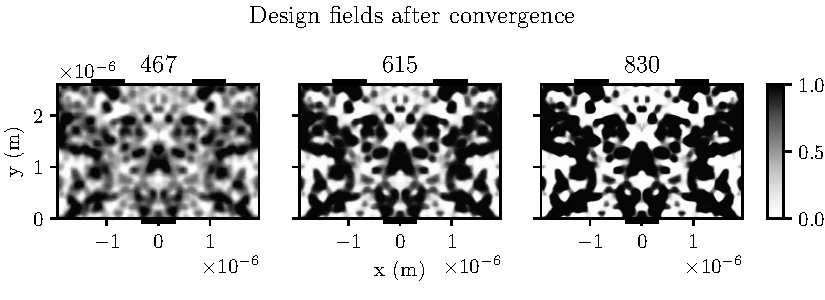
\includegraphics{chapters/results/interpolation_fields_468615830.pdf}
	\caption{This figure shows the interpolation field at iteration 467, 615,
		and 830. It is clearly seen that the device becomes closer and closer to
		being binary.
	}%
	\label{fig:cont_design1}
\end{figure}

\section{Level-set optimization}\label{sec:res_bin}

% Because the continuous optimization didn't converge until rather late,
% I did not have time to explore the level-set optimization as much as I would
% have liked.
The initial contour of the device was taken as the 0.5-isocontour of the final
design field from the continuous optimization.
\Cref{fig:bin_conv} shows the convergence plot for the level-set optimization,
and \cref{fig:bin_design} shows the final device.
Something to note is that the device does seem to be rather sensitive;
a shift of only a nanometre can greatly change the device performance.
Therefore the $\alpha$ chosen for the algorithm had to be set as low as
\qty{0.5}{\nm}.

\begin{figure}[htpb]
	\centering
	\includegraphics{chapters/results/conv_tmp.pdf}
	\caption{Still running simulation :D}%
	\label{fig:bin_conv}
\end{figure}

\begin{figure}[htpb]
	\centering
	\includegraphics{chapters/results/bin_design_tmp_254.pdf}
	\caption{%
		The current best design from the level-set simulations (but they are
		still running:)
	}%
	\label{fig:bin_design}
\end{figure}

\chapter{Concluding Remarks}

Phononics have the potential to become a vital part of both quantum  and
classical information processing architecture, but devices are still limited to
those that can be investigated through analytical means and/or be optimized with
brute force methods. This study set out to investigate whether inverse design
with adjoint simulation could be used to design so far unrealized devices and
enable little explored applications.

I first examined theoretically the applicability of adjoint simulation on
phononics, from which I concluded that the methods should work in theory.
The second aim of this thesis was to demonstrate the utility of this method by
designing a phononic beamsplitter.
To do that, the process was split into two stages, a first where the material
was allowed to vary continuously, and a second where a binary design was
enforced using level-set methods.
The continuous optimization yielded near perfect performance, validating the
theoretical derivations.
The level-set optimization never did achieve perfect performance, but
good performance was still reached.
These results indicate that the inverse design concept can be very useful for
designing phononic devices going forward.
We remain hopeful that the problems with the latter stage can be solved
though, which would be a major step forward.

\section{Future Research}

There are a great number of potential paths that can be explored from this
point, and the positive results presented here warrant further efforts in this
area.
One important improvement that should be investigated is the sensitivity of the
device to small changes in the design.
If it is very sensitive, imperfections in fabrication could be detrimental to
the devices performance.
There may be some ways of mitigating this however, for example by running
multiple simulations with small perturbations in the design and averaging them
to obtain the objective function.
Another potential path of exploration is the limiting of the feature size.
This could be done by augmenting the objective function, adding
a pure part that punishes small features.

In addition to method improvements, another path is to apply this to designing
other types of devices. For example, waveguide bends seem to be well suited for
this type of design, and would be useful if one wishes to use phononic
waveguides for routing excitations around on a chip. It may also be possible to
inverse design hybrid devices that use both optics and mechanics for example,
though that would likely require a significant effort.


% REFERENCES / BIBLIOGRAPHY
\include{template/pages/bibliography}

% APPENDICES
% \cleardoublepage
% \appendix
% \pagenumbering{bychapter}
% \include{appendices/first_appendix}

% LAST PAGE
\if\thesisStatus f
    \include{template/pages/lastpage}
\fi

\end{document}
